\section{What a loop is worth on text}
\label{sec:text}

\subsection{The pre-registered law cannot say what a loop is worth}
\label{sec:verdicts}

The pre-registration measured the value of a loop by one number per loop type: the exponent $\varphi$ of
$\Neff = \Nonce + r^{\varphi}\Nrec$, read off a dense ruler fitted to the grid's 54 dense results (one result per run
and budget). Five model sizes were
too few for this. The ruler puts its irreducible loss at the lowest value the fit allowed ($E = 0.050$) and its parameter
exponent at $\alpha = 0.054$, far below the usual value of about 0.3, because five sizes cannot pin down $E$, $A$ and
$\alpha$ separately. $\varphi$ inherits this weakness: it is 0--0.17 per loop type with the primary fit, and 0--0.41 with the joint fit over all 352 results (two of the grid's results are excluded;
Appendix~\ref{app:prereg}), which gives $\alpha = 0.267$ (Table~\ref{tab:prereg}).

Under the pre-registered decision rules, none of the four hypotheses held as stated. Table~\ref{tab:prereg} gives the verdicts and
Appendix~\ref{app:prereg} the details. For example, truncated backpropagation was predicted to lower $\varphi$ (H1). With truncation, $\varphi$ was lower in the middle block, though the intervals
overlap, and higher in the whole stack, where truncation also lowered the loss of the whole stack looped 4 times at every size.
Truncated runs also had most of the loss spikes (Appendix~\ref{app:training}).

Fitted separately at each size against the same ruler, and allowed to be negative, $\varphi$ of the 4-loop model is
$-0.32$, 0.19, 0.39, 0.52 and 0.65 from 10M to 160M \lbl{(exploratory)}. These values come from the same weak ruler, so we use only their direction: the value of a
loop rises with model size, and a single $\varphi$ per loop type averages over very different regimes. The rest of this
section therefore measures the value of a loop without a fitted law.

\begin{table}[t]
  \centering
  \caption{Pre-registered results. Top: $\varphi$ per loop type on the main validation set (equal-token accounting, $N$
  including the output head), from the primary analysis with 95\% block-bootstrap intervals and from the secondary joint fit; both fits bound
  $\varphi$ below by 0. Bottom: the verdicts on the four hypotheses under the frozen decision rules (in full in
  Table~\ref{tab:verdicts}).}
  \label{tab:prereg}
  \footnotesize
  \begin{tabular}{lcc}
    \toprule
    Loop type & $\varphi$, primary [95\% interval] & $\varphi$, joint fit \\
    \midrule
    Middle block, full backpropagation & 0.13 [0.02, 0.27] & 0.41 \\
    Middle block, truncated            & 0.00 [0.00, 0.17] & 0.29 \\
    Whole stack, full backpropagation  & 0.00 [0.00, 0.16] & 0.00 \\
    Whole stack, truncated             & 0.17 [0.10, 0.20] & 0.29 \\
    \bottomrule
  \end{tabular}

  \vspace{0.5em}
  \begin{tabular}{>{\raggedright\arraybackslash}p{0.56\linewidth}>{\raggedright\arraybackslash}p{0.38\linewidth}}
    \toprule
    Hypothesis & Verdict \\
    \midrule
    H1: truncation lowers $\varphi$ & Not supported \\
    H2: a middle block has a higher $\varphi$ than the whole stack & Depends on the measure \\
    H3: the gain from loops saturates in $r$ & Not supported \\
    H4: the best $r$ is small at equal training compute, larger at equal deployment compute & First half trivially (dense is best); second not supported \\
    \bottomrule
  \end{tabular}
\end{table}

\subsection{Measured directly, a loop's value rises with model size and data}
\label{sec:multiplier}

\begin{figure}[t]
  \centering
  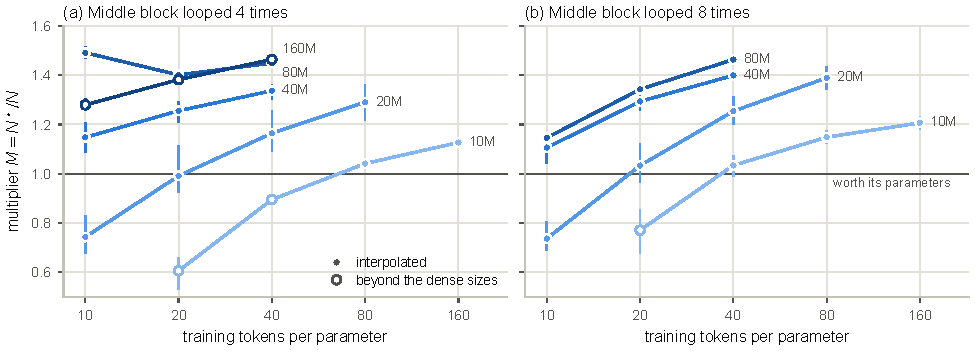
\includegraphics[width=\linewidth]{fig2_multiplier}
  \caption{What each parameter of a middle-block looped model is worth in dense parameters: the multiplier
  $M = \Nstar/N$. $\Nstar$ is the size of the dense model that reaches the same loss on the same number of training
  tokens, interpolated between the measured dense sizes (including the dense models trained longer in S4,
  Section~\ref{sec:equalcompute}). $M = 1$: as good as a dense model of its own size. Open markers: $\Nstar$ lies beyond
  the largest or smallest dense size, by at most a factor of two. Diamonds: dense models with 18 layers and about the
  looped model's number of parameters (Section~\ref{sec:depth}). Bars: 95\% intervals from resampling the seeds (three; two at
  160M; one at 80M), a rough guide with so few seeds.}
  \label{fig:multiplier}
\end{figure}

The dense runs themselves can serve as the ruler. For each looped model, we read the loss of every measured dense size
at the looped model's number of training tokens, and interpolate the dense size $\Nstar$ that has the same loss. The
multiplier $M = \Nstar/N$ is then what each parameter of the looped model is worth in dense parameters
(Figure~\ref{fig:multiplier}, \lbl{exploratory}).

For the 4-loop model, $M$ depends on size and data. At 10M--20M with 10--20 tokens per
parameter, $M$ is 0.6--1.0 where it can be read: the looped model is worth at most a dense model of its own size. At 40M--160M with 20--40 tokens per
parameter, $M$ is 1.26--1.46. For some of these values, $\Nstar$ lies outside the measured dense sizes, by less than a
factor of two: below the smallest for the 10M value of 0.6, and above the largest for the 160M values. At 10M with 10 tokens per parameter, $M$ is not reported: the looped model is worse than both dense models
measured at that number of tokens, and these two are out of order (the 20M one, trained on 5.7 tokens per parameter,
is worse than the 10M one), so the dense size of equal loss cannot be extrapolated (Appendix~\ref{app:fits}).

$M$ rises with data at 10M--40M and at 160M. At 80M, with one seed, it is flat:
1.49, 1.40 and 1.45 at $10N$, $20N$ and $40N$. Fitting $\log_2 M$ as a plane in $\log_2 N$ and $\log_2$(tokens per parameter) gives a factor of 1.21 per
doubling of model size and 1.14 per doubling of tokens per parameter (Appendix~\ref{app:fits}). Looping 8 times
instead of 4 raises $M$ by up to 0.16 at 10M--20M (0.11 among the values within the measured dense sizes), with no
consistent change from 40M on.

$M$ counts all of $N$, including the output head, which lies outside the looped block (34\% of $N$ at 10M, 21\% at
40M). The local exponent $\varphi_{\mathrm{loc}}$ credits the whole gain to the looped parameters; it is negative where
$M < 1$ ($-0.84$ at 20M with 10 tokens per parameter) and 0.22--0.55 from 40M on. If $N$ excludes the head, as in
\citet{schwethelm2026how}, $\varphi_{\mathrm{loc}}$ is 0.32--0.50 at 40M--160M with 20--40 tokens per parameter, close
to their $\varphi = 0.46$ (Appendix~\ref{app:fits}).

The shared learning rate does not create this trend. A supplementary experiment (S1, \lbl{pre-specified};
Appendix~\ref{app:lr}) re-tuned the learning rates of the dense model and the 4-loop model at 10M--40M, with one seed
(two at 20M). Re-tuning changed the gap between them by at most 0.005 nats at 20M--40M. At 10M, where the looped
model preferred lower rates, it improved the looped model's standing by about 0.02 nats. With each model at its best
rate, the size trend at $40N$ is somewhat smaller but meets the plan's criterion, which asks that it keep more than half of its value at the shared rate. The data trend at 10M is larger than at the shared rate: the gap goes from $+0.082$ at $10N$ to $-0.059$ at
$160N$.

Converted to $M$, the equal-parameter results of Parcae \citep{prairie2026parcae} and Ouro \citep{zhu2025scaling}
reach a similar level (1.23--1.46 at 134M--770M), but not the same trend: Parcae's values fall with size at about 80
tokens per parameter, and Ouro's rise with size while its tokens per parameter fall. The shallower looped blocks of
\citet{saunshi2025reasoning}, trained on about 750--1500 tokens per parameter, reach 1.47--1.95
(Appendix~\ref{app:published}). The published results barely sample models below 40M trained on 20 or fewer tokens per parameter, where we find the looped model worth at most a dense model of its own size. A value that rises with tokens per parameter is not captured by effective-parameter laws in which the factor applied to
the looped parameters does not depend on the training tokens \citep{schwethelm2026how,chen2026moe}.

Every dense model of this ruler has eight layers, while the 4-loop model executes 20. At a fixed size, deeper and thinner
models do better below a billion parameters \citep{liu2024mobilellm}, though the shape matters little over a wide range
of shapes \citep{kaplan2020scaling}. So $M$ may measure what depth gives at a fixed size rather than what sharing gives.

\subsection{At 40M, a deeper dense model of the same size recovers about half of the loop's advantage}
\label{sec:depth}

To separate depth from sharing, a supplementary experiment (S10, \lbl{pre-specified}) trained dense models with 18 layers and about the looped model's number of parameters: 18 layers of
width 320 ($N = 28.1$M) at 20M and of width 448 ($N = 51.2$M) at 40M. Their executed depth of 18 is close to the 4-loop model's 20. They use the grid's recipe, data, budgets and three
seeds. Their learning rate follows the grid's rule
(Section~\ref{sec:grid}): the embedding and output layers use the rate of their width, and the hidden layers use
$(18/12)^{-1/2}$ times it. We call this the
rule's rate. Their multiplier $M_{\mathrm{deep}}$ is read off the same 8-layer dense runs and compared with the 4-loop model's
multiplier $M_{\mathrm{loop}}$ at the same size and budget. The plan fixed in advance how to interpret them. It defines
$R = \log M_{\mathrm{deep}} / \log M_{\mathrm{loop}}$, computed at 40M for each budget and averaged over the three
budgets, as the share of the looped model's advantage that a dense model of the same size and nearly the same
depth recovers. The plan reads $R \geq 0.75$ as ``most of the advantage is a depth effect'', $0.25 \leq R < 0.75$ as ``partly depth, partly sharing'' and $R < 0.25$ as ``looping buys more than depth''.

At 40M, the deep dense model is worth 1.10, 1.11 and 1.11 dense parameters
per parameter at $10N$, $20N$ and $40N$; the looped model is worth 1.15, 1.26 and 1.34 (Figure~\ref{fig:multiplier}a,
diamonds). So $R$ is 0.50 (0.41--0.62 when the three seeds are resampled), in the band the plan reads as ``partly depth, partly sharing'', as it predicted. At 40M, the value of depth does not grow with data, but the looped model's lead
over the deep model does. The lead is 0.003 nats at $10N$, 0.015 at $20N$ and 0.029 at $40N$, with the same sign in all three seeds
at the two longer budgets. At 20M, the deep model is narrow (width 320) and worse than the 8-layer model of the same size
($M_{\mathrm{deep}} = 0.84$--0.94). There, depth explains none of the looped model's advantage at $40N$
($M_{\mathrm{loop}} = 1.16$; the plan reports 20M descriptively).

The deep model's learning rate was
checked with one seed (seed 42). At 40M its best rate was the highest one tried, 1.41 times the rule's rate, at all three budgets, beating the rule's rate by 0.014, 0.006 and 0.001 nats at $10N$, $20N$ and $40N$. Because it beat the rule's rate by more than 0.01 nats at $10N$, the plan asks for a second
computation with each model at its best tested rate (Appendix~\ref{app:s10}). Computed that way, the deep model is ahead of the looped one
at $10N$ by 0.010 nats ($M = 1.37$ against 1.18, so $R = 1.91$), and $R$ is 0.56 and 0.34 at $20N$ and $40N$ (0.45 and
0.37 for the same seed at the rule's rate). These readings may understate the deep model, because its
best rate lies at the edge of the range tried and the plan had no rule to extend the range. Their average, 0.94, would count as ``most of the advantage is a depth effect''. But this average is dominated by the $10N$ value, where $\log M_{\mathrm{loop}}$ is only 0.17 and the ratio is
unstable, and the plan keeps the value at the rule's rate as the primary result. The deep model also costs about half the training compute of the
looped model: 406M against 835M FLOPs per token at 40M.

About half of the looped model's advantage at equal parameters at 40M thus comes from depth. With each model at its best tested learning rate, depth accounts for all of it at the shortest budget, in the one seed
tried:
the deep model's lead there, 0.010 nats, is twice the range of this gap across the three seeds at the rule's rate
(Table~\ref{tab:s10}). At 20M depth explains none of the advantage, and at neither size does depth recover the
part that grows with data (Appendix~\ref{app:s10}).

\subsection{At equal training compute, the dense model wins all but one measured comparison}
\label{sec:equalcompute}

At equal parameters, a middle block looped 2, 4 or 8 times costs 1.4--1.5, 2.2--2.4 or 3.7--4.1 times the training FLOPs
per token of the dense model. For an equal-compute comparison, we give the dense model the tokens it could have seen
with the looped run's compute, and read its loss off the measured dense curve \lbl{(exploratory)}.

\begin{figure}[t]
  \centering
  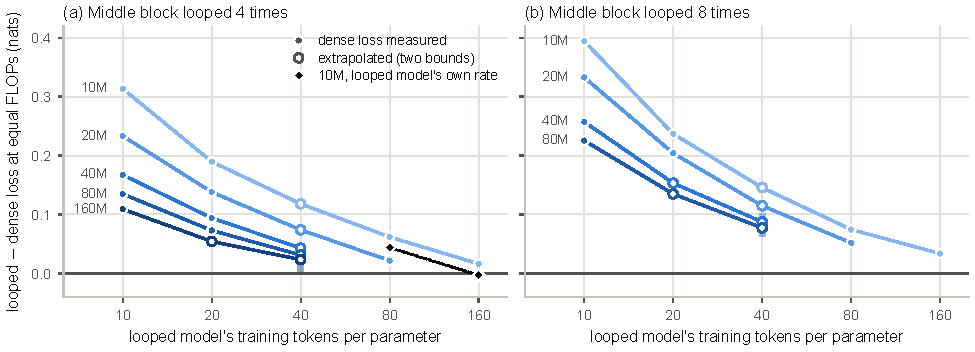
\includegraphics[width=\linewidth]{fig3_equal_compute}
  \caption{Equal training compute: looped minus dense loss, when the dense model of the same size is trained on the
  tokens that the looped run's compute would buy (positive: dense better). Filled markers: the dense loss is measured,
  including the dense models trained longer in S4, to $640N$ (10M) and $320N$ (20M). Open markers with bars: the dense loss is
  extrapolated, and the bar spans the two extrapolations (from the power law to the extended last segment). Diamonds: the 10M model looped 4 times,
  trained at 0.35 times the dense rate, the lowest rate S1 tried (mean of two seeds; bars: seed range).}
  \label{fig:equalcompute}
\end{figure}

The grid and its extensions have 320 looped results. For 221 of them, the original dense runs reach the equal-compute
point, and at the shared learning rate the dense model won all of them, by at least 0.016 nats. Continuing the 10M dense models to $640N$ and the 20M ones to $320N$ (S4, \lbl{pre-specified})
turned 37 more comparisons into measured ones (Figure~\ref{fig:equalcompute}), and the dense model won these as well:
all 258 measured comparisons at the shared rate. These comparisons share dense curves, trunks and seeds, so they are not
independent.

The dense model's lead shrinks with data: for the 10M 4-loop model trained on $40N$, $80N$ and $160N$, it is $+0.119$ nats (with the dense loss extrapolated for one seed), $+0.062$ and $+0.016$. Table~\ref{tab:equalcompute} in Appendix~\ref{app:lr} lists the comparisons at the
largest budgets.

The remaining comparisons need an extrapolated dense loss, which two extrapolations bound: a power law fitted to
each dense curve, which favours looping, and an extension of the curve's last measured segment, which favours the dense model (Appendix~\ref{app:lr}). Of the 99 such comparisons before S4, looping came out ahead in 6 under the
power law, by at most 0.021 nats, all at the largest data per parameter. Where S4 measured such comparisons, the measured gaps fall about
halfway between the two extrapolations; 62 comparisons remain extrapolated.

With each model at its best tested learning rate (S1),
the dense model won 10 of the 11 comparisons (one of them, 40M at $40N$, on an extrapolated dense loss). The eleventh is
at 10M and $160N$, with the looped model at 0.35 times the dense rate. That was the lowest rate tried, and the looped
model's loss was still falling as the rate went down. There the two are level on average ($-0.011$ and $+0.005$ in two
seeds). It is the only measured equal-compute comparison in this study that the dense model does not win.

The deep dense models of Section~\ref{sec:depth} cost about half the looped model's compute per token, and they are ahead by 0.11--0.19 nats wherever their measured curves reach the equal-compute point \lbl{(exploratory)}.

\subsection{At deployment, the loop saves some weight memory but costs decoding time and KV cache for every executed
layer}
\label{sec:cost}

We measured inference on one RTX 4090 in bf16, with KV-cached decoding and a separate cache for every executed layer, so that decoding computes what the models
computed in training (S3, \lbl{pre-specified}; Appendix~\ref{app:cost}). At these sizes, decoding time follows
the number of executed layers. At equal parameters, a middle block looped 2, 4 or 8 times takes 1.5, 2.4--2.6 or
4.5--4.6 times the decoding time per token of the dense model, close to the ratios of executed layers.

At equal quality, the comparison is with the dense model that reaches the same loss when both are trained on 40
tokens per parameter, interpolated between the measured dense sizes. This differs from $\Nstar$, which holds the number
of training tokens fixed. Against it, the 4-loop
model needs less weight memory: 4\% less at 20M, rising to 19\% at 160M, where the dense model of equal loss is
extrapolated. But it needs 2.20--2.41 times the KV cache per token, 2.37--2.47 times the decoding time and about 1.6
times the peak memory at batch 32.

One way to cut this cost is to share the KV cache across loops. Each core layer then keeps one cache for all loops,
and every loop reads the earlier tokens' keys and values as they were written at those tokens' last loop. This would
remove most of the cache and memory cost, though not the decoding time. A supplementary experiment (S6, \lbl{pre-specified}) applied it after
training to 20M models of one seed, at the constant-rate checkpoint at $32N$ from which the $40N$ cooldown branches
off. The models include a 4-loop model trained at half the dense rate in S1. The comparison with the dense model at
the same checkpoint and on the same tokens was added after a review and is \lbl{exploratory}
(Appendix~\ref{app:deviations}). For every model that gains
from its loops, sharing costs 2.2 to 7.4 times that gain (0.09--0.17 nats, against gains of 0.019--0.046 over the dense
model), so each would end up worse than the dense model of its size. These gains come from one seed, and at 20M the
gap between a looped and a dense model varies across seeds by 0.032--0.045 nats (Section~\ref{sec:measurement}), so
the ratios are rough. By the S6 plan's thresholds (an increase above 0.02 nats ``degrades'', above 0.1
``breaks''), sharing degrades the 8-loop model (by
0.09 nats) and breaks the truncated 8-loop model (0.14), the 4-loop model (0.17) and, at the boundary, the 4-loop
model at half the rate (0.10; Appendix~\ref{app:cost}). Sharing costs nothing only for the models trained with a random loop count, whose block
contracts to a fixed point (Section~\ref{sec:mechanism}); these models gain nothing over the dense model. We tested neither of two routes that may avoid this cost: training the loop to converge, and
training with a shared cache from the start. \citet{monea2026shared} pretrain looped models with a scheme in which only the first loop
writes the cache, and find that it costs no quality in their setting.

\paragraph{What the loop buys on text.} Where the loop helps at equal parameters, it saves parameters and data but costs compute. From about 40M to 160M,
with 20--40 tokens per parameter, each parameter of the 4-loop model is worth about 1.3--1.5 dense parameters, more with more data at most sizes. At 40M, a dense model of the same size and nearly the same depth gets about half of that advantage for half the
compute (all of it at the shortest budget once its learning rate is tuned, in one seed), but not the part that grows
with data. At equal training compute the dense model wins every measured
comparison but one, and at deployment the loop costs decoding time and KV cache for every executed layer. The next two sections test the second
claim: that running more loops at inference solves harder problems.
